\chapter{Genética de poblaciones y selección natural}\label{ch:b2:population-genetics}

En 1848 se capturó cerca de Mánchester una polilla del abedul negra; en
1895, diecinueve de cada veinte polillas de la ciudad eran negras, y hacia
1970, a medida que desaparecía el hollín, había vuelto la forma clara. Las
polillas no cambiaron: cambiaron las proporciones de dos \omterm{def:b2:meiosis-heredity:vocabulary}{alelos} en una
población de millones, bajo la mirada de las aves, en unas pocas decenas
de generaciones. Darwin había visto que la selección debía cambiar las
especies, pero no tenía manera de contarlo; ese recuento es la \omterm{def:b2:population-genetics:frequencies}{genética de
poblaciones}, y es la aritmética de este capítulo. Se pregunta cómo se
comportan las \omterm{def:b2:population-genetics:frequencies}{frecuencias alélicas} cuando nada actúa sobre ellas, y
después con qué rapidez las desplazan la selección, la \omterm{def:b2:genome-diversification:mutation}{mutación}, la
migración, el azar y la endogamia --- y termina con los caracteres que no
dependen de un gen sino de muchos, que son la mayor parte de lo que la
selección ve realmente.

\section{El acervo génico en reposo}

\begin{definition}[Población, acervo génico, frecuencias]\label{def:b2:population-genetics:frequencies}
\index{genética de poblaciones}\index{acervo génico}\index{frecuencia alélica}
Una \emph{población} es un grupo de individuos de una especie que se
cruzan entre sí; su \emph{acervo génico} es el conjunto de todos sus
\omterm{def:b2:meiosis-heredity:vocabulary}{alelos}. Para un locus con dos \omterm{def:b2:meiosis-heredity:vocabulary}{alelos} $A$ y $a$ en una población \omterm{def:b2:meiosis-heredity:meiosis}{diploide}
de $N$ individuos, las \emph{frecuencias alélicas} son $p = (2N_{AA} +
N_{Aa})/2N$ y $q = 1 - p$, y las \emph{frecuencias genotípicas} son las
proporciones de $AA$, $Aa$ y $aa$. La evolución, en su sentido más
estricto, es un cambio de las frecuencias alélicas entre generaciones; la
pregunta de este capítulo es qué las cambia y cuánto.
\end{definition}

\begin{theorem}[Hardy--Weinberg]\label{thm:b2:population-genetics:hw}
\index{ley de Hardy--Weinberg}
En una población grande con apareamiento aleatorio, sin selección,
\omterm{def:b2:genome-diversification:mutation}{mutación} ni migración, las \omterm{def:b2:population-genetics:frequencies}{frecuencias alélicas} no cambian de una
generación a la siguiente y, tras una sola generación de apareamiento
aleatorio, las frecuencias genotípicas son
\[
AA : p^{2}, \qquad Aa : 2pq, \qquad aa : q^{2},
\]
y se mantienen así. La dominancia no hace que un \omterm{def:b2:meiosis-heredity:vocabulary}{alelo} \omterm{def:b2:meiosis-heredity:vocabulary}{dominante} se
extienda, y un \omterm{def:b2:meiosis-heredity:vocabulary}{alelo} \omterm{def:b2:meiosis-heredity:vocabulary}{recesivo} raro no se pierde: se esconde en los
\omterm{def:b2:meiosis-heredity:vocabulary}{heterocigotos}, que superan en número a los \omterm{def:b2:meiosis-heredity:vocabulary}{homocigotos} en una proporción
de $2p/q$ a uno --- para $q = 0.01$, doscientos a uno. La ley es la
hipótesis nula de la \omterm{def:b2:population-genetics:frequencies}{genética de poblaciones}: una desviación respecto de
ella en una población real, o un cambio de
$p$ entre generaciones, es la huella de una de las fuerzas que siguen.
\end{theorem}
\begin{proof}
El apareamiento aleatorio es la unión aleatoria de gametos: un gameto
porta $A$ con probabilidad $p$ y $a$ con probabilidad $q$, con
independencia de su pareja, de modo que el cigoto es $AA$ con probabilidad
$p^{2}$, $Aa$ con $2pq$ y $aa$ con $q^{2}$. La \omterm{def:b2:population-genetics:frequencies}{frecuencia alélica} en la
generación siguiente es $p' = p^{2} + \tfrac12(2pq) = p(p + q) = p$: sin
cambios. Como las frecuencias genotípicas solo dependen de $p$, son las
mismas en todas las generaciones posteriores a la primera.
\end{proof}

\begin{example}[Leer una frecuencia]\label{ex:b2:population-genetics:cf}
La fibrosis quística, recesiva, afecta a uno de cada 2500 niños europeos:
$q^{2} = 1/2500$, $q = 0.02$, y la frecuencia de portadores es $2pq
\approx 0.04$ --- una persona de cada 25 porta un \omterm{def:b2:meiosis-heredity:vocabulary}{alelo} que mata a sus
\omterm{def:b2:meiosis-heredity:vocabulary}{homocigotos}, y el \qty{98}{\%} de las copias del \omterm{def:b2:meiosis-heredity:vocabulary}{alelo} se encuentran en
portadores sanos, donde la selección no puede verlas. Por eso un \omterm{def:b2:meiosis-heredity:vocabulary}{recesivo}
letal se elimina tan despacio, y por eso los proyectos eugenésicos de
eliminar las enfermedades recesivas esterilizando a los afectados nunca
habrían podido funcionar: la aritmética de la sección siguiente muestra
con qué lentitud.
\end{example}

\section{La selección}

\begin{definition}[Eficacia biológica]\label{def:b2:population-genetics:fitness}
\index{eficacia biológica}\index{coeficiente de selección}
La \emph{eficacia biológica} $w$ de un \omterm{def:b2:meiosis-heredity:vocabulary}{genotipo} es su contribución
relativa en descendientes a la generación siguiente --- la supervivencia
hasta la reproducción por la fecundidad ---, escalada de modo que el mejor
\omterm{def:b2:meiosis-heredity:vocabulary}{genotipo} tenga $w = 1$. El \emph{coeficiente de selección} $s$ de un
\omterm{def:b2:meiosis-heredity:vocabulary}{genotipo} es su déficit,
$w = 1 - s$. La eficacia biológica es una propiedad de un \omterm{def:b2:meiosis-heredity:vocabulary}{genotipo} en un
ambiente, no de un \omterm{def:b2:meiosis-heredity:vocabulary}{alelo} en sí mismo: el \omterm{def:b2:meiosis-heredity:vocabulary}{alelo} de la polilla melánica
tenía $w > 1$ respecto del claro sobre la \omterm{def:b2:plant-meristems:wood}{corteza} cubierta de hollín y
$w < 1$ sobre los líquenes.
\end{definition}

\begin{theorem}[La selección cambia la frecuencia alélica]\label{thm:b2:population-genetics:selection}
\index{selección natural!ecuación}
Con eficacias genotípicas $w_{AA}$, $w_{Aa}$, $w_{aa}$, la eficacia media
es $\bar w = p^{2}w_{AA} + 2pq\,w_{Aa} + q^{2}w_{aa}$ y la \omterm{def:b2:population-genetics:frequencies}{frecuencia
alélica} en la generación siguiente es
\[
p' = \frac{p^{2}w_{AA} + pq\,w_{Aa}}{\bar w}, \qquad
\Delta p = p' - p = \frac{pq\,\bigl[p(w_{AA} - w_{Aa}) + q(w_{Aa} - w_{aa})\bigr]}{\bar w}.
\]
Dos consecuencias. En primer lugar, $\Delta p$ es proporcional a $pq$: la
selección es más rápida a frecuencias intermedias y más lenta cuando un
\omterm{def:b2:meiosis-heredity:vocabulary}{alelo} es raro o está casi fijado --- hay poca variación sobre la que
actuar. En segundo lugar, contra un \omterm{def:b2:meiosis-heredity:vocabulary}{alelo} \omterm{def:b2:meiosis-heredity:vocabulary}{recesivo} ($w_{AA} = w_{Aa} = 1$, $w_{aa} =
1 - s$) el cambio es $\Delta q = -s\,pq^{2}/\bar w$, proporcional
a $q^{2}$: un \omterm{def:b2:meiosis-heredity:vocabulary}{recesivo} raro es casi invisible para la selección, y reducir
a la mitad su frecuencia desde $0.01$ lleva unas cien generaciones
incluso cuando sus \omterm{def:b2:meiosis-heredity:vocabulary}{homocigotos} son letales. Un \omterm{def:b2:meiosis-heredity:vocabulary}{alelo} \omterm{def:b2:meiosis-heredity:vocabulary}{dominante} favorable
se extiende deprisa al principio y después se estanca al final, por la
misma razón.
\end{theorem}
\begin{proof}
De los descendientes, una fracción $p^{2}w_{AA}/\bar w$ son $AA$ y
$2pq\,w_{Aa}/\bar w$ son $Aa$ (la frecuencia de cada \omterm{def:b2:meiosis-heredity:vocabulary}{genotipo} ponderada
por su eficacia y renormalizada); los \omterm{def:b2:meiosis-heredity:vocabulary}{alelos} $A$ entre ellos son todos los
del primero y la mitad de los del segundo, lo que da $p'$. Restando $p =
p\bar w/\bar w$ y desarrollando $\bar w$ se obtiene $\Delta p$. Para un
\omterm{def:b2:meiosis-heredity:vocabulary}{recesivo} letal ($s = 1$): $q' = q^{2}\cdot 0 + pq$ dividido por $\bar w = 1 -
q^{2}$, de modo que $q' = q/(1 + q)$, luego $1/q' = 1/q + 1$ y al cabo de $t$
generaciones $1/q_t = 1/q_0 + t$: pasar de $q_0 = 0.01$ a $0.005$ lleva
$t = 100$.
\end{proof}

\begin{omfigure}
\begin{tikzpicture}
\begin{axis}[
  width=0.8\linewidth, height=6cm,
  axis x line=bottom, axis y line=left,
  xmin=0, xmax=150, ymin=0, ymax=1.05,
  xlabel={generaciones}, ylabel={frecuencia del alelo favorecido},
  xlabel style={font=\small, at={(axis description cs:0.5,-0.11)}, anchor=north},
  ylabel style={font=\small},
  tick label style={font=\small}, xtick={0,50,100,150}, ytick={0,0.5,1},
  legend style={font=\scriptsize, at={(0.97,0.35)}, anchor=east, draw=none},
  clip=false,
]
\addplot[very thick, omDef] table[x=t, y=dom] {
t dom
0 0.01
10 0.02
20 0.04
30 0.075
40 0.14
50 0.24
60 0.38
70 0.53
80 0.66
90 0.76
100 0.83
110 0.88
120 0.91
130 0.93
140 0.945
150 0.955
};
\addlegendentry{alelo favorecido dominante, $s = 0.1$}
\addplot[very thick, omThm] table[x=t, y=rec] {
t rec
0 0.01
10 0.0101
20 0.0102
30 0.0104
40 0.0106
50 0.0108
60 0.011
70 0.0113
80 0.0116
90 0.012
100 0.0124
110 0.0128
120 0.0133
130 0.0138
140 0.0144
150 0.015
};
\addlegendentry{alelo favorecido recesivo, $s = 0.1$}
\end{axis}
\end{tikzpicture}

{\small La selección en acción con una ventaja del \qty{10}{\%}. Un \omterm{def:b2:meiosis-heredity:vocabulary}{alelo}
\omterm{def:b2:meiosis-heredity:vocabulary}{dominante} favorecido pasa del \qty{1}{\%} a la mayoría en setenta
generaciones y después se frena, porque su rival \omterm{def:b2:meiosis-heredity:vocabulary}{recesivo}, ya raro, se
esconde en los \omterm{def:b2:meiosis-heredity:vocabulary}{heterocigotos}; un \omterm{def:b2:meiosis-heredity:vocabulary}{alelo} \omterm{def:b2:meiosis-heredity:vocabulary}{recesivo} favorecido al \qty{1}{\%}
apenas se mueve en el mismo tiempo, puesto que casi nunca queda expuesto.}
\end{omfigure}

\begin{proposition}[Tipos de selección]\label{prop:b2:population-genetics:kinds}
\index{selección direccional}\index{selección estabilizadora}\index{selección equilibradora}\index{ventaja del heterocigoto}
La selección \emph{direccional} favorece un extremo y lleva un \omterm{def:b2:meiosis-heredity:vocabulary}{alelo}
hacia la fijación (la polilla melánica en un bosque cubierto de hollín; la
resistencia a los antibióticos; el tamaño del pico de un pinzón durante
una sequía). La selección
\emph{estabilizadora} favorece el valor intermedio y elimina los extremos
(el peso al nacer en la especie humana: los bebés que mueren son los más
pequeños y los más grandes); mantiene la población donde está y es el tipo
más común. La selección \emph{disruptiva} favorece los dos extremos frente
al valor intermedio, y puede dividir una población
(\cref{ch:b2:speciation}). La selección \emph{equilibradora} mantiene dos
\omterm{def:b2:meiosis-heredity:vocabulary}{alelos} en la población de forma indefinida: por \emph{\omterm{prop:b2:population-genetics:kinds}{ventaja del
heterocigoto}}, cuando $Aa$ es más apto que cualquiera de los \omterm{def:b2:meiosis-heredity:vocabulary}{homocigotos}
--- con
$w_{AA} = 1 - s$, $w_{aa} = 1 - t$, $w_{Aa} = 1$, la frecuencia se
estabiliza en $\hat p = t/(s + t)$ --- o por selección \emph{dependiente de
la frecuencia}, cuando un \omterm{def:b2:meiosis-heredity:vocabulary}{genotipo} es más apto cuanto más raro es (los
\omterm{def:b2:meiosis-heredity:vocabulary}{alelos} $S$ raros del \cref{ch:b2:angiosperm-reproduction}, las presas que
un depredador no ha aprendido a reconocer, los dos lados de la boca de un
pez que come escamas).
\end{proposition}
\begin{proof}[Evidencia]
La hemoglobina falciforme mata a la mayoría de los \omterm{def:b2:meiosis-heredity:vocabulary}{homocigotos} antes de
que se reproduzcan, y sin embargo el \omterm{def:b2:meiosis-heredity:vocabulary}{alelo} está entre el \qty{10}{\%} y el
\qty{20}{\%} en toda el África palúdica. Allison (1954) demostró que los
niños \omterm{def:b2:meiosis-heredity:vocabulary}{heterocigotos} sufrían infecciones palúdicas mucho menos numerosas y
más leves que cualquiera de los \omterm{def:b2:meiosis-heredity:vocabulary}{homocigotos}, y la frecuencia del \omterm{def:b2:meiosis-heredity:vocabulary}{alelo} se
superpone a la distribución histórica del paludismo por falciparum; en las
poblaciones de ascendencia africana que viven donde no hay paludismo, la
frecuencia no ha dejado de bajar desde entonces. Con $t \approx 0.8$ para
el \omterm{def:b2:meiosis-heredity:vocabulary}{homocigoto} falciforme y $s \approx 0.1$ para el \omterm{def:b2:meiosis-heredity:vocabulary}{homocigoto} normal en
una región palúdica,
$\hat q = s/(s + t) \approx 0.11$ --- lo que se observa.
\end{proof}

\section{Mutación, migración y equilibrio}

\begin{theorem}[Equilibrio mutación--selección]\label{thm:b2:population-genetics:balance}
\index{equilibrio mutación--selección}\index{carga genética}
Un \omterm{def:b2:meiosis-heredity:vocabulary}{alelo} perjudicial es alimentado por la \omterm{def:b2:genome-diversification:mutation}{mutación} a una tasa $\mu$ por
gameto y por generación y eliminado por la selección. En el equilibrio,
ambas se compensan: para un \omterm{def:b2:meiosis-heredity:vocabulary}{alelo} \omterm{def:b2:meiosis-heredity:vocabulary}{recesivo} con una desventaja homocigótica
$s$,
\[
\hat q = \sqrt{\mu/s}\,;
\]
para un \omterm{def:b2:meiosis-heredity:vocabulary}{alelo} \omterm{def:b2:meiosis-heredity:vocabulary}{dominante} (o parcialmente \omterm{def:b2:meiosis-heredity:vocabulary}{dominante}) con una desventaja
heterocigótica $hs$, $\hat q = \mu/hs$. La frecuencia de equilibrio de un
\omterm{def:b2:meiosis-heredity:vocabulary}{recesivo} es, por tanto, grande incluso para un letal: con $\mu = 10^{-5}$ y
$s = 1$, $\hat q = 3\times 10^{-3}$, y el \qty{0.6}{\%} de la población lo
porta. Toda población soporta una \emph{\omterm{thm:b2:population-genetics:balance}{carga genética}} de este tipo en
miles de loci, en su mayor parte recesiva y oculta, y el equilibrio del
argumento del trinquete del \cref{ch:b2:asexual-reproduction}
--- una fracción $e^{-U/s}$ de individuos libres de \omterm{def:b2:genome-diversification:mutation}{mutaciones}
perjudiciales --- es el mismo equilibrio sumado sobre todo el genoma.
\end{theorem}
\begin{proof}
En cada generación, la \omterm{def:b2:genome-diversification:mutation}{mutación} añade $\mu p \approx \mu$ a $q$ y la
selección retira $s\,pq^{2}/\bar w \approx sq^{2}$ (para $q$ pequeña);
igualando $\mu = s\hat q^{2}$ se obtiene el resultado \omterm{def:b2:meiosis-heredity:vocabulary}{recesivo}. Para un
\omterm{def:b2:meiosis-heredity:vocabulary}{alelo} \omterm{def:b2:meiosis-heredity:vocabulary}{dominante}, la selección retira $hs\,q$ por generación (cada copia
queda expuesta en un \omterm{def:b2:meiosis-heredity:vocabulary}{heterocigoto}), y $\mu = hs\hat q$.
\end{proof}

\begin{proposition}[La migración y la regla de un migrante]\label{prop:b2:population-genetics:migration}
\index{flujo génico}\index{migración (genética)}
Si una fracción $m$ de una población está formada en cada generación por
inmigrantes procedentes de una población con \omterm{def:b2:population-genetics:frequencies}{frecuencia alélica} $p_{m}$,
la frecuencia se desplaza hacia $p_{m}$ en $\Delta p = m(p_{m} - p)$: la
diferencia entre las dos poblaciones decae como $(1 - m)^{t}$. El
\emph{\omterm{prop:b2:population-genetics:migration}{flujo génico}} homogeneiza; deshace la \omterm{def:b2:plant-plasticity:plasticity}{adaptación} local a menos que
la selección sea más fuerte que $m$, y es la fuerza que mantiene una
especie como una sola especie. A la inversa, las poblaciones que no
intercambian migrantes divergen por deriva y por sus \omterm{def:b2:genome-diversification:mutation}{mutaciones} propias, y
un solo migrante por generación --- sea cual sea el tamaño de la
población --- basta para impedir que la deriva las lleve a fijar \omterm{def:b2:meiosis-heredity:vocabulary}{alelos}
distintos.
\end{proposition}

\section{El azar: la deriva genética}

\begin{theorem}[Deriva genética]\label{thm:b2:population-genetics:drift}
\index{deriva genética}\index{tamaño efectivo de la población}\index{fijación}
En una población de $N$ individuos \omterm{def:b2:meiosis-heredity:meiosis}{diploides}, la \omterm{def:b2:population-genetics:frequencies}{frecuencia alélica} de
cada generación es una muestra aleatoria de $2N$ gametos de la anterior,
de modo que $p$ fluctúa al azar con una varianza de
$p(1 - p)/2N$ por generación. La \emph{heterocigosidad} $H = 2pq$
disminuye por término medio en un factor $(1 - 1/2N)$ en cada generación,
\[
H_t = H_0\left(1 - \frac{1}{2N}\right)^{t} \approx H_0\,e^{-t/2N},
\]
y todo \omterm{def:b2:meiosis-heredity:vocabulary}{alelo} acaba perdiéndose o \emph{fijándose}, con una probabilidad
igual a su frecuencia actual: una nueva \omterm{def:b2:genome-diversification:mutation}{mutación} neutra, a frecuencia
$1/2N$, se fija con probabilidad $1/2N$ y, si lo hace, tarda unas $4N$
generaciones. La deriva es despreciable en una población de millones y
\omterm{def:b2:meiosis-heredity:vocabulary}{dominante} en una de decenas: un \emph{cuello de botella} o un
acontecimiento \emph{fundador} --- unos pocos colonos en una isla, una
especie reducida a cien individuos por la caza --- pierde \omterm{def:b2:meiosis-heredity:vocabulary}{alelos} por azar
en una generación y deja una población uniforme, empobrecida y llena de
\omterm{def:b2:meiosis-heredity:vocabulary}{homocigotos}. El $N$ que importa es el tamaño \emph{efectivo}, el número de
individuos que se reproducen realmente, normalmente muy inferior al del
censo.
\end{theorem}
\begin{proof}
Las $2N$ copias génicas de la generación siguiente se extraen con
reposición de un acervo en el que $A$ tiene frecuencia $p$: el número de
copias $A$ sigue una binomial de media $2Np$ y varianza $2Np(1 - p)$, de
modo que $p'$ tiene media $p$ y varianza $p(1 - p)/2N$. Dos copias tomadas
al azar en la generación siguiente proceden de la misma copia parental con
probabilidad $1/2N$ y son entonces idénticas, de modo que la probabilidad
de que dos copias difieran (la heterocigosidad) se multiplica por
$1 - 1/2N$ en cada generación. Probabilidad de fijación: la frecuencia de
un \omterm{def:b2:meiosis-heredity:vocabulary}{alelo} neutro es una martingala --- su valor esperado nunca cambia --- y
termina en 0 o en 1, de modo que la probabilidad de terminar en 1 es igual
a su valor inicial.
\end{proof}
\begin{omfigure}
\begin{tikzpicture}
\begin{axis}[
  width=0.82\linewidth, height=6cm,
  axis x line=bottom, axis y line=left,
  xmin=0, xmax=60, ymin=0, ymax=1.05,
  xlabel={generaciones}, ylabel={frecuencia alélica $p$},
  xlabel style={font=\small, at={(axis description cs:0.5,-0.11)}, anchor=north},
  ylabel style={font=\small},
  tick label style={font=\small}, xtick={0,20,40,60}, ytick={0,0.5,1},
  legend style={font=\scriptsize, at={(0.5,-0.25)}, anchor=north, draw=none, legend columns=2},
  clip=false,
]
\addplot[thick, omThm] coordinates {(0,0.5) (2,0.55) (4,0.62) (6,0.58) (8,0.7) (10,0.8) (12,0.75) (14,0.85) (16,0.92) (18,0.88) (20,0.95) (22,1) (60,1)};
\addlegendentry{$N = 10$}
\addplot[thick, omThm!60] coordinates {(0,0.5) (2,0.42) (4,0.35) (6,0.4) (8,0.3) (10,0.2) (12,0.25) (14,0.15) (16,0.1) (18,0.05) (20,0.08) (22,0.02) (24,0) (60,0)};
\addplot[thick, omDef] coordinates {(0,0.5) (5,0.52) (10,0.49) (15,0.53) (20,0.56) (25,0.54) (30,0.58) (35,0.55) (40,0.57) (45,0.6) (50,0.58) (55,0.61) (60,0.6)};
\addlegendentry{$N = 1000$}
\addplot[thick, omDef!60] coordinates {(0,0.5) (5,0.48) (10,0.5) (15,0.47) (20,0.45) (25,0.46) (30,0.44) (35,0.45) (40,0.43) (45,0.44) (50,0.42) (55,0.43) (60,0.42)};
\end{axis}
\end{tikzpicture}

{\small La deriva. Dos poblaciones de diez individuos que parten de
$p = 0.5$ fijan \omterm{def:b2:meiosis-heredity:vocabulary}{alelos} opuestos en veinticinco generaciones; dos de mil
individuos fluctúan unos pocos puntos porcentuales en sesenta.}
\end{omfigure}

\begin{proposition}[La endogamia]\label{prop:b2:population-genetics:inbreeding}
\index{endogamia}\index{coeficiente de endogamia}\index{depresión endogámica}
El apareamiento entre parientes no cambia las \omterm{def:b2:population-genetics:frequencies}{frecuencias alélicas}, pero
eleva la proporción de \omterm{def:b2:meiosis-heredity:vocabulary}{homocigotos}: el \emph{\omterm{prop:b2:population-genetics:inbreeding}{coeficiente de endogamia}} $F$
de un individuo es la probabilidad de que sus dos \omterm{def:b2:meiosis-heredity:vocabulary}{alelos} en un locus sean
idénticos por ascendencia, y las frecuencias genotípicas pasan a ser
$p^{2} + Fpq$, $2pq(1 - F)$, $q^{2} + Fpq$. Para los
hijos de primos hermanos, $F = 1/16$; de hermanos, $1/4$; de
autofecundación, $1/2$. Como los \omterm{def:b2:meiosis-heredity:vocabulary}{alelos} \omterm{def:b2:meiosis-heredity:vocabulary}{recesivos} de la \omterm{thm:b2:population-genetics:balance}{carga genética}
quedan expuestos en los \omterm{def:b2:meiosis-heredity:vocabulary}{homocigotos} adicionales, los descendientes
endogámicos sufren \emph{\omterm{prop:b2:population-genetics:inbreeding}{depresión endogámica}}: un \omterm{def:b2:meiosis-heredity:vocabulary}{recesivo} letal a
$q = 0.01$ aparece en $q^{2} = 10^{-4}$ de los descendientes de
apareamientos aleatorios, pero en
$q^{2} + Fpq = 7\times 10^{-4}$ de los hijos de primos, siete veces más;
sumada sobre miles de loci, la mortalidad infantil de los hijos de primos
es aproximadamente el doble que la de los demás, y una población pequeña
que practica la endogamia durante generaciones pierde fertilidad y vigor
--- la situación del guepardo, de la pantera de Florida y de las casas
reales de Europa.
\end{proposition}

\section{Muchos genes: los caracteres cuantitativos}

\begin{theorem}[La heredabilidad y la respuesta a la selección]\label{thm:b2:population-genetics:heritability}
\index{heredabilidad}\index{genética cuantitativa}\index{ecuación del criador}
Un carácter como la estatura, el rendimiento de un cultivo o la
profundidad del pico depende de muchos genes de efecto pequeño y del
ambiente, y varía de forma continua. Su varianza en una población se
divide en una parte \emph{genética} $V_G$ y una parte \emph{ambiental}
$V_E$, y la \emph{heredabilidad} $h^{2} = V_A/V_P$ es la fracción de la
varianza fenotípica debida a los efectos aditivos de los genes (la parte
que se transmite). Si los progenitores de la generación siguiente se
seleccionan con una media que supera la de la población en $S$ (el
\emph{diferencial de selección}), su descendencia la supera en
\[
R = h^{2}\,S
\]
--- la \emph{\omterm{thm:b2:population-genetics:heritability}{ecuación del criador}}. Es toda la mejora animal y vegetal en
una línea: una heredabilidad de $0.5$ y unos progenitores situados una
desviación típica por encima de la media dan una descendencia situada
media desviación típica por encima, y la ganancia se acumula generación
tras generación. La heredabilidad es una propiedad de una población en un
ambiente, no de un carácter: no dice nada sobre si un rasgo es inmutable,
y un rasgo con $h^{2} = 0.8$ en una población puede tener
$h^{2} = 0$ en otra en la que todos los individuos tienen el mismo
\omterm{def:b2:meiosis-heredity:vocabulary}{genotipo}.
\end{theorem}
\begin{proof}
El \omterm{def:b2:meiosis-heredity:vocabulary}{fenotipo} esperado de la descendencia se regresa sobre el del
progenitor medio con pendiente $h^{2}$ (la covarianza genética aditiva
entre parientes dividida por la varianza fenotípica), de modo que una
desviación parental $S$ da una desviación de la descendencia $h^{2}S$. En
la práctica, $h^{2}$ se mide a partir de esa regresión, o del parecido
entre gemelos y hermanos, o de la propia respuesta.
\end{proof}
\begin{proof}[Evidencia]
El experimento del maíz de Illinois, iniciado en 1896, seleccionó cada año
las mazorcas con el contenido de aceite más alto y más bajo: al cabo de
cien generaciones, la línea alta había pasado del \qty{5}{\%} al
\qty{20}{\%} de aceite y la línea baja había caído por debajo del
\qty{1}{\%}, y ambas seguían respondiendo --- la variación de muchos genes
no se agota en un siglo de selección. En las Galápagos, los Grant midieron
todos los pinzones de una isla durante la sequía de 1977: los
supervivientes tenían picos un \qty{4}{\%} más profundos que los muertos,
el carácter tenía $h^{2}
\approx 0.7$, y los polluelos del año siguiente tenían picos un
\qty{3}{\%} más profundos que los de la generación anterior --- una
selección observada, medida y cuya respuesta predijo la ecuación
anterior.
\end{proof}

\begin{omfigure}
\begin{tikzpicture}
\begin{axis}[
  width=0.78\linewidth, height=5.6cm,
  axis x line=bottom, axis y line=left,
  xmin=6, xmax=14, ymin=0, ymax=0.32,
  xlabel={profundidad del pico (mm)}, ylabel={frecuencia},
  xlabel style={font=\small, at={(axis description cs:0.5,-0.12)}, anchor=north},
  ylabel style={font=\small},
  tick label style={font=\small}, xtick={7,9,11,13}, ytick=\empty,
  legend style={font=\scriptsize, at={(0.5,-0.28)}, anchor=north, draw=none, legend columns=3},
  clip=false,
]
\addplot[very thick, omDef, domain=6:14, samples=100] {0.3*exp(-((x-9.4)^2)/(2*0.9))};
\addlegendentry{antes de la sequía, media 9,4}
\addplot[very thick, omThm, domain=6:14, samples=100] {0.28*exp(-((x-9.9)^2)/(2*0.8))};
\addlegendentry{supervivientes, media 9,9}
\addplot[very thick, omProp, dashed, domain=6:14, samples=100] {0.3*exp(-((x-9.75)^2)/(2*0.9))};
\addlegendentry{generación siguiente, media 9,75}
\draw[<->] (axis cs:9.4,0.02) -- (axis cs:9.9,0.02); \node[font=\scriptsize, anchor=south] at (axis cs:9.65,0.025) {$S$};
\end{axis}
\end{tikzpicture}

{\small La \omterm{thm:b2:population-genetics:heritability}{ecuación del criador} en una población de pinzones. La sequía
dejó supervivientes con un pico medio $S = \qty{0.5}{mm}$ más profundo;
con $h^{2} = 0.7$, su descendencia tenía el pico $R = \qty{0.35}{mm}$ más
profundo que la generación anterior.}
\end{omfigure}

\begin{example}[La aritmética de la polilla]\label{ex:b2:population-genetics:moth}
El \omterm{def:b2:meiosis-heredity:vocabulary}{alelo} melánico de la polilla del abedul es \omterm{def:b2:meiosis-heredity:vocabulary}{dominante}. Pasar de una
frecuencia de alrededor de $10^{-3}$ en 1848 al \qty{90}{\%} de polillas
melánicas (una frecuencia cercana a $0.7$) en 1895 son cincuenta
generaciones; la ecuación de la selección lo reproduce con un $s$ de
entre $0.2$ y $0.3$ contra la forma clara
--- y los experimentos de liberación de Kettlewell en la década de 1950,
en los que las aves capturaban las polillas claras sobre troncos cubiertos
de hollín y las oscuras sobre troncos limpios aproximadamente en esa
proporción, midieron directamente el coeficiente. El regreso tras las
leyes de aire limpio, del \qty{90}{\%} de melánicas en 1960 a menos del
\qty{10}{\%} en 2000, avanzó a la misma velocidad en sentido contrario.
Todo el episodio --- una población grande, un \omterm{def:b2:meiosis-heredity:vocabulary}{alelo} \omterm{def:b2:meiosis-heredity:vocabulary}{dominante}, un agente
selectivo fuerte y reversible --- es la \omterm{def:b2:population-genetics:frequencies}{genética de poblaciones}
desarrollándose a la vista de todos.
\end{example}

\begin{omfigure}
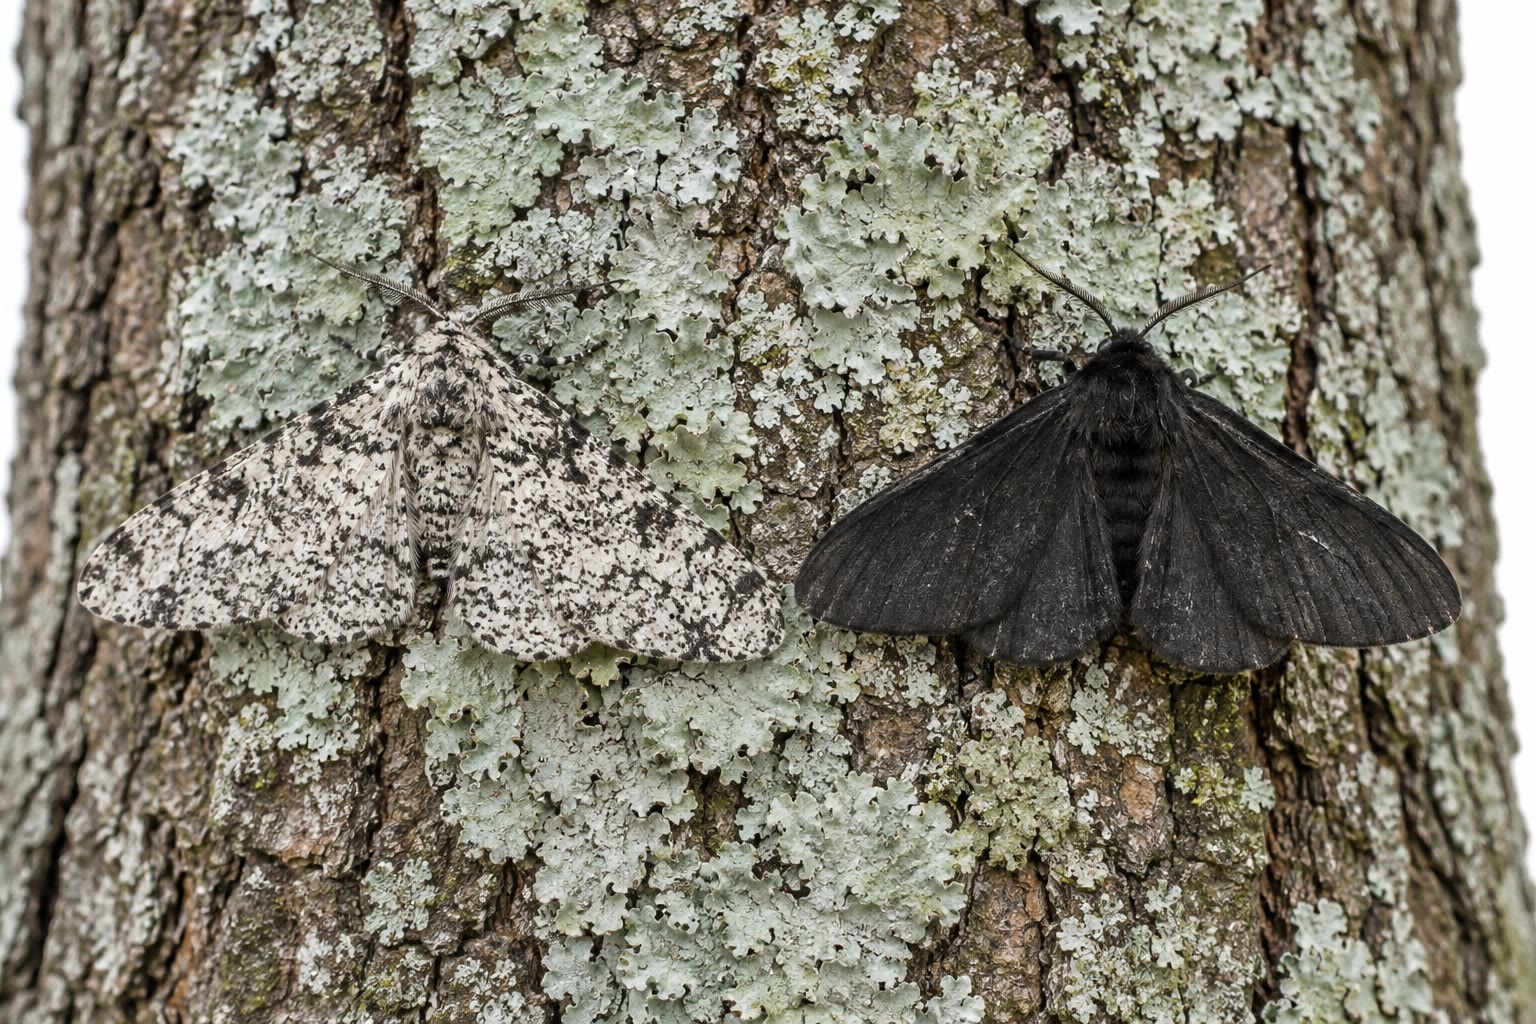
\includegraphics[width=0.46\linewidth]{images/book4/ai/b4-22-peppered-moths.jpg}\hspace{0.04\linewidth}
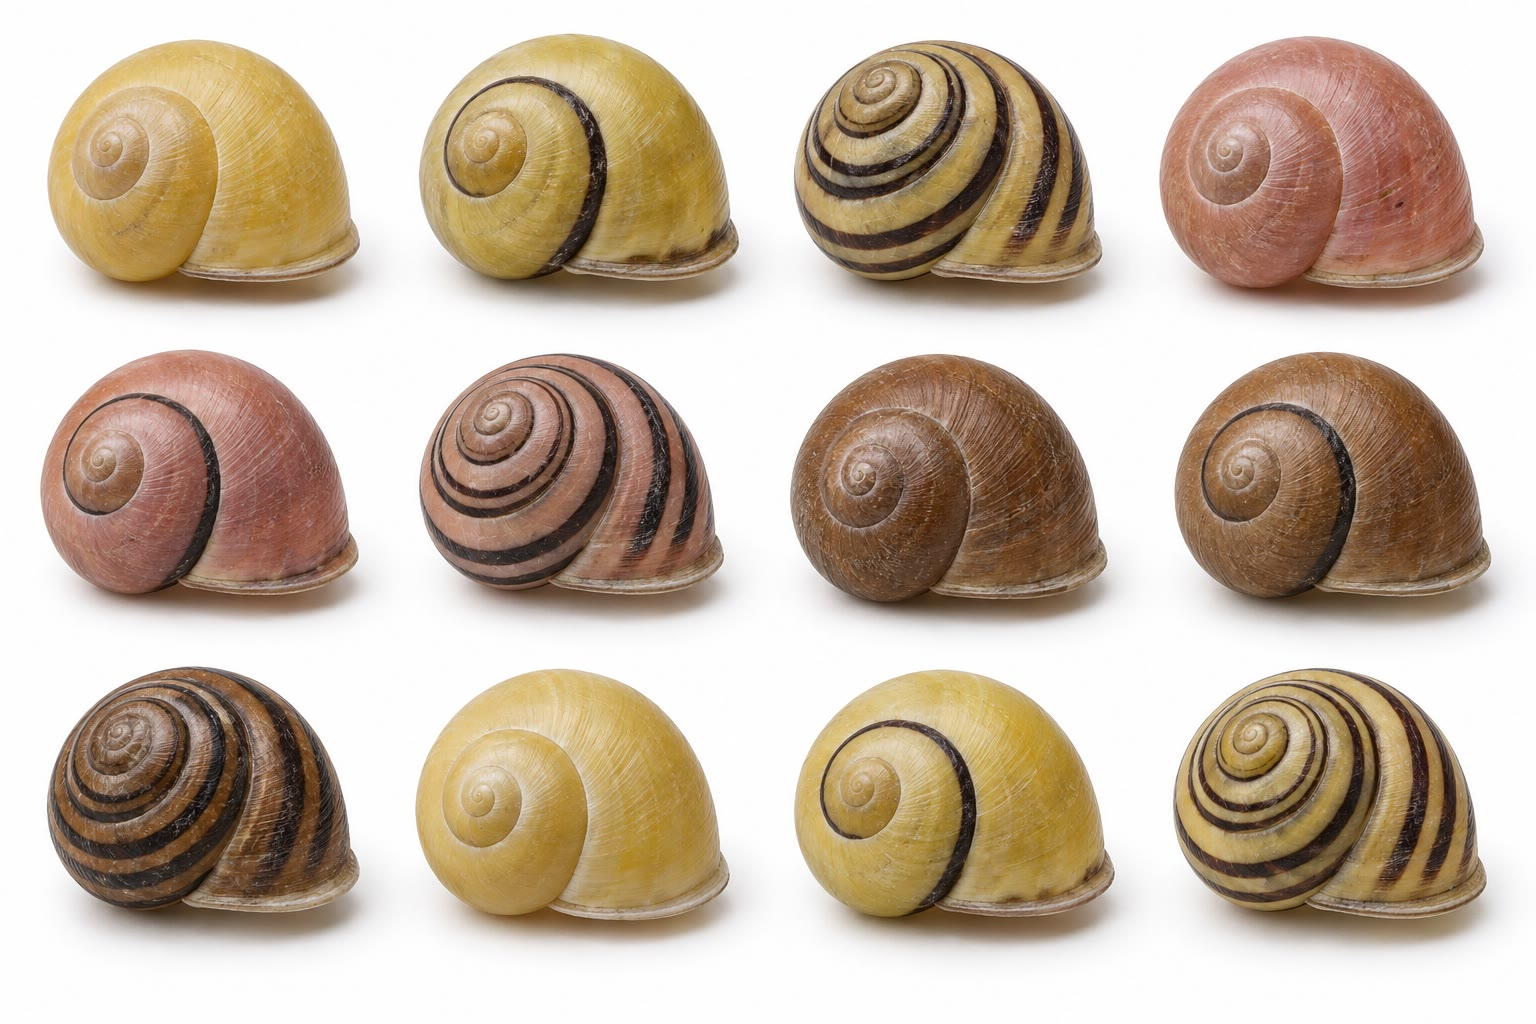
\includegraphics[width=0.46\linewidth]{images/book4/ai/b4-22-banded-snails.jpg}

{\small Izquierda: las dos formas de la polilla del abedul sobre
líquenes --- cuál encuentra un ave depende de la \omterm{def:b2:plant-meristems:wood}{corteza}. Derecha: el
polimorfismo de la concha del caracol de bosque, con colores y bandas que
se mantienen en todas las poblaciones gracias a depredadores que aprenden
a reconocer la forma común.}
\end{omfigure}

\section{Ejercicios}

\begin{exercise}[$\star$]\label{exo:b2:population-genetics:1}
En una muestra de 1000 personas, 640 son $MM$, 320 $MN$ y 40 $NN$.
Calcúlense las \omterm{def:b2:population-genetics:frequencies}{frecuencias alélicas} y las proporciones esperadas de
Hardy--Weinberg. ¿Está la población en equilibrio?
\end{exercise}

\begin{exercise}[$\star$]\label{exo:b2:population-genetics:2}
El albinismo es \omterm{def:b2:meiosis-heredity:vocabulary}{recesivo} y afecta a una persona de cada \num{20000}.
Calcúlense la \omterm{def:b2:population-genetics:frequencies}{frecuencia alélica} y la frecuencia de portadores.
\end{exercise}

\begin{exercise}[$\star$]\label{exo:b2:population-genetics:3}
Defínanse \omterm{def:b2:population-genetics:fitness}{eficacia biológica}, \omterm{def:b2:population-genetics:fitness}{coeficiente de selección} y heredabilidad, y
dense las cinco fuerzas que cambian las \omterm{def:b2:population-genetics:frequencies}{frecuencias alélicas}.
\end{exercise}

\begin{exercise}[$\star$]\label{exo:b2:population-genetics:4}
Dese un ejemplo de \omterm{prop:b2:population-genetics:kinds}{selección direccional}, uno de estabilizadora y uno de
equilibradora, con el agente de selección en cada caso.
\end{exercise}

\begin{exercise}[$\star\star$]\label{exo:b2:population-genetics:5}
Un \omterm{def:b2:meiosis-heredity:vocabulary}{alelo} \omterm{def:b2:meiosis-heredity:vocabulary}{recesivo} letal tiene una frecuencia de $0.02$. ¿Cuántas
generaciones hacen falta para reducirla a la mitad? ¿Y para llegar a
$0.001$? ¿Qué dice esto sobre el efecto de impedir que los individuos
afectados se reproduzcan?
\end{exercise}

\begin{exercise}[$\star\star$]\label{exo:b2:population-genetics:6}
Con $w_{AA} = 1$, $w_{Aa} = 1$, $w_{aa} = 0.8$ y $p = 0.3$, calcúlense
$\bar w$, $p'$ y $\Delta p$. Repítase para $p = 0.9$. ¿Por qué el
segundo cambio es mucho menor?
\end{exercise}

\begin{exercise}[$\star\star$]\label{exo:b2:population-genetics:7}
En una región palúdica, el \omterm{def:b2:meiosis-heredity:vocabulary}{homocigoto} falciforme tiene $w = 0.2$ y el
\omterm{def:b2:meiosis-heredity:vocabulary}{homocigoto} normal
$w = 0.88$, y los \omterm{def:b2:meiosis-heredity:vocabulary}{heterocigotos} $w = 1$. Calcúlense la frecuencia de
equilibrio del \omterm{def:b2:meiosis-heredity:vocabulary}{alelo} falciforme y la fracción de niños que nacen con la
enfermedad en el equilibrio.
\end{exercise}

\begin{exercise}[$\star\star$]\label{exo:b2:population-genetics:8}
Un letal \omterm{def:b2:meiosis-heredity:vocabulary}{recesivo} surge por \omterm{def:b2:genome-diversification:mutation}{mutación} a $\mu = \qty{2e-5}{}$ por gameto.
Calcúlense su frecuencia de equilibrio y la fracción de nacimientos
afectados. Un letal \omterm{def:b2:meiosis-heredity:vocabulary}{dominante} (antes de la reproducción) a la misma tasa:
¿qué fracción de los nacimientos?
\end{exercise}

\begin{exercise}[$\star\star$]\label{exo:b2:population-genetics:9}
Una población de 50 individuos reproductores parte de $H = 0.5$.
Calcúlese su heterocigosidad al cabo de 10, 50 y 200 generaciones. ¿Qué
tamaño debe tener una población para conservar el \qty{90}{\%} de su
heterocigosidad durante 100 generaciones?
\end{exercise}

\begin{exercise}[$\star\star\star$]\label{exo:b2:population-genetics:10}
Una isla es colonizada por 10 aves procedentes de una población
continental en la que un \omterm{def:b2:meiosis-heredity:vocabulary}{alelo} tiene una frecuencia de $0.1$. Calcúlense
la probabilidad de que el \omterm{def:b2:meiosis-heredity:vocabulary}{alelo} esté ausente en los fundadores y la
probabilidad de que acabe fijándose en la isla si está presente en una
sola copia. Compárese con el continente.
\end{exercise}

\begin{exercise}[$\star\star\star$]\label{exo:b2:population-genetics:11}
La producción de leche tiene $h^{2} = 0.3$ y una desviación típica de
\qty{1000}{L}. Un criador conserva como madres el \qty{20}{\%} superior de
las vacas (cuya media está $1.4$ desviaciones típicas por encima de la del
rebaño). Calcúlese la respuesta por generación. Si los toros se eligen
entre el \qty{1}{\%} superior (media $2.7$ desviaciones típicas por
encima), ¿cuál es la respuesta? ¿Por qué se frena la respuesta tras muchas
generaciones?
\end{exercise}

\begin{exercise}[$\star\star\star$]\label{exo:b2:population-genetics:12}
``La selección es ciega a lo que no puede ver.'' Discútase, con el \omterm{def:b2:meiosis-heredity:vocabulary}{alelo}
\omterm{def:b2:meiosis-heredity:vocabulary}{recesivo} en los \omterm{def:b2:meiosis-heredity:vocabulary}{heterocigotos}, la \omterm{def:b2:genome-diversification:mutation}{mutación} neutra y el carácter de
heredabilidad nula, sobre qué puede actuar la selección y sobre qué no.
\end{exercise}

\section{Problema: la polilla, la isla y el rebaño}

\begin{problem}[{Problema de fin de semana --- el ascenso de la polilla del
abedul calculado con la ecuación de la selección, la deriva y la endogamia
de una población fundadora seguidas en el tiempo, un equilibrio
mutación--selección establecido y un programa de mejora predicho, hasta
llegar al coeficiente de selección de la polilla, la heterocigosidad de la
isla y la ganancia del rebaño}]
\label{pb:b2:population-genetics:1}
Polilla del abedul: \omterm{def:b2:meiosis-heredity:vocabulary}{alelo} melánico $M$ \omterm{def:b2:meiosis-heredity:vocabulary}{dominante}, frecuencia $p_0 = 0.001$
en 1848; \qty{90}{\%} de polillas melánicas 50 generaciones más tarde;
supóngase
$w_{MM} = w_{Mm} = 1$ y $w_{mm} = 1 - s$. Isla: fundada por 12 aves de un
continente donde $H = 0.4$ y un \omterm{def:b2:meiosis-heredity:vocabulary}{alelo} \omterm{def:b2:meiosis-heredity:vocabulary}{recesivo} perjudicial tiene
$q = 0.05$; después la isla alberga 40 aves reproductoras. \omterm{def:b2:genome-diversification:mutation}{Mutación}:
$\mu = \qty{1e-5}{}$. Rebaño: $h^{2} = 0.4$, desviación típica de
\qty{800}{L}.

\medskip
\noindent\textbf{Parte I --- La polilla.}
\begin{enumerate}
  \item En 1848, ¿qué fracción de las polillas era melánica, y qué
        fracción de los \omterm{def:b2:meiosis-heredity:vocabulary}{alelos} $M$ se encontraba en \omterm{def:b2:meiosis-heredity:vocabulary}{heterocigotos}?
  \item Demuéstrese que, con $M$ \omterm{def:b2:meiosis-heredity:vocabulary}{dominante}, la frecuencia del \omterm{def:b2:meiosis-heredity:vocabulary}{alelo} claro
        cumple $q' = q(1 - sq)/(1 - sq^{2})$.
  \item Partiendo de $q_0 = 0.999$, calcúlese $q$ al cabo de una generación
        para $s = 0.3$.
  \item Un \qty{90}{\%} de melánicas significa $q^{2} = 0.1$. ¿Cuánto vale
        entonces $q$?
  \item Por tanteo con la recurrencia (o con la aproximación
        $\Delta q \approx -sq^{2}p$ mientras $q$ está cerca de 1), estímese
        el número de generaciones necesarias con $s = 0.3$ para llevar $q$
        de $0.999$ a $0.32$, y compárese con las 50 observadas.
  \item Tras las leyes de aire limpio, la forma clara tiene la ventaja: $s
        = 0.3$ contra $mm$ pasa a ser $s = 0.3$ contra $M\_$. Demuéstrese
        que $\Delta p = -spq^{2}/\bar w$, y explíquese por qué el regreso
        de la forma clara es lento al principio y termina en un descenso
        exponencial de $M$, mientras que el ascenso empezó de forma
        exponencial y terminó arrastrándose.
\end{enumerate}

\medskip
\noindent\textbf{Parte II --- La isla.}
\begin{enumerate}[resume]
  \item Calcúlese la probabilidad de que ninguno de los 12 fundadores porte
        el \omterm{def:b2:meiosis-heredity:vocabulary}{alelo} perjudicial.
  \item Calcúlese la heterocigosidad esperada tras la generación fundadora
        (extraída de $H = 0.4$ por 12 individuos, es decir, 24 copias
        génicas).
  \item Calcúlese la heterocigosidad al cabo de 100 generaciones con $N =
        40$, como fracción de la del continente.
  \item Aparece una \omterm{def:b2:genome-diversification:mutation}{mutación} neutra en un ave. Calcúlense su probabilidad
        de fijación y el tiempo esperado hasta la fijación si se fija.
  \item Las aves de la isla se aparean al azar, pero todas están
        emparentadas. Con un $F = 1/(2N)$ que se acumula en cada generación
        hasta alrededor de $0.3$ al cabo de 30 generaciones, calcúlese la
        frecuencia de \omterm{def:b2:meiosis-heredity:vocabulary}{homocigotos} afectados para el \omterm{def:b2:meiosis-heredity:vocabulary}{alelo} con $q = 0.05$,
        con y sin endogamia.
  \item Llega un ave del continente en cada generación. Explíquese qué
        efecto tiene esto sobre la divergencia de la isla y sobre su carga.
\end{enumerate}

\medskip
\noindent\textbf{Parte III --- El equilibrio.}
\begin{enumerate}[resume]
  \item Calcúlense la frecuencia de equilibrio de un letal \omterm{def:b2:meiosis-heredity:vocabulary}{recesivo}
        alimentado por $\mu = 10^{-5}$ y la fracción de nacimientos
        afectados.
  \item Calcúlese lo mismo para $s = 0.1$ (un \omterm{def:b2:meiosis-heredity:vocabulary}{recesivo} ligeramente
        perjudicial).
  \item Calcúlese el equilibrio para un \omterm{def:b2:meiosis-heredity:vocabulary}{alelo} \omterm{def:b2:meiosis-heredity:vocabulary}{dominante} con una desventaja
        heterocigótica $hs = 0.05$.
  \item La medicina cura el letal, de modo que $s$ baja a $0.1$. ¿Cómo
        cambia el equilibrio, y cuánto tiempo (en orden de magnitud) tarda
        la población en alcanzarlo?
  \item El genoma tiene \num{20000} genes, cada uno de los cuales muta a un
        letal \omterm{def:b2:meiosis-heredity:vocabulary}{recesivo} a una tasa de $10^{-5}$. ¿Cuántos \omterm{prop:b2:meiosis-heredity:extensions}{alelos letales}
        porta en estado \omterm{def:b2:meiosis-heredity:vocabulary}{heterocigoto} una persona media? (En el equilibrio,
        cada locus tiene $2\hat q$ copias por persona.)
  \item Explíquese por qué ese número es compatible con una población sana
        y por qué hace costosos los matrimonios entre primos.
\end{enumerate}

\medskip
\noindent\textbf{Parte IV --- El rebaño.}
\begin{enumerate}[resume]
  \item El criador conserva el \qty{30}{\%} superior de las vacas (media
        $1.16$ desviaciones típicas por encima del rebaño). Calcúlense el
        diferencial de selección en litros y la respuesta.
  \item Tras cinco generaciones de la misma selección, ¿cuál es la
        ganancia esperada, y por qué podría ser menor la ganancia real?
  \item Los toros aportan la mitad de los genes y se seleccionan entre el
        \qty{2}{\%} superior ($2.4$ desviaciones típicas). Calcúlese la
        respuesta cuando las vacas y los toros se seleccionan como se ha
        indicado (promédiense los dos diferenciales).
  \item Un rebaño en el que todas las vacas son \omterm{def:b2:asexual-reproduction:clone}{clones} de un mismo animal:
        ¿cuánto valen $h^{2}$ y la respuesta? ¿Qué dice esto sobre la
        heredabilidad?
  \item Una población de pinzones tiene $h^{2} = 0.7$ para la profundidad
        del pico, y la sequía deja supervivientes con picos \qty{0.6}{mm}
        más profundos. Predígase la generación siguiente.
  \item El criador pasa a un rasgo con $h^{2} = 0.1$. ¿Qué diferencial de
        selección, en desviaciones típicas, da la misma respuesta que en la
        pregunta 19?
  \item Enúnciese el resultado: el $s$ de la polilla y el tiempo hasta el
        \qty{90}{\%} de melánicas, la heterocigosidad de la isla al cabo de
        100 generaciones y la respuesta del rebaño por generación.
\end{enumerate}
\end{problem}
